%%%%%%%%%%%%%%%%%%%%%%%%%%%%%%%%%%%%%%%%%
% Beamer Presentation
% LaTeX Template
% Version 1.0 (10/11/12)
%
% This template has been downloaded from:
% http://www.LaTeXTemplates.com
%
% License:
% CC BY-NC-SA 3.0 (http://creativecommons.org/licenses/by-nc-sa/3.0/)
%
%%%%%%%%%%%%%%%%%%%%%%%%%%%%%%%%%%%%%%%%%

%----------------------------------------------------------------------------------------
%	PACKAGES AND THEMES
%----------------------------------------------------------------------------------------

\documentclass{beamer}

\mode<presentation> {

% The Beamer class comes with a number of default slide themes
% which change the colors and layouts of slides. Below this is a list
% of all the themes, uncomment each in turn to see what they look like.

%\usetheme{default}
%\usetheme{AnnArbor}
%\usetheme{Antibes}
%\usetheme{Bergen}
%\usetheme{Berkeley}
%\usetheme{Berlin}
%\usetheme{Boadilla}
%\usetheme{CambridgeUS}
%\usetheme{Copenhagen}
%\usetheme{Darmstadt}
%\usetheme{Dresden}
%\usetheme{Frankfurt}
%\usetheme{Goettingen}
%\usetheme{Hannover}
%\usetheme{Ilmenau}
%\usetheme{JuanLesPins}
%\usetheme{Luebeck}
%\usetheme{Madrid}
%\usetheme{Malmoe}
%\usetheme{Marburg}
%\usetheme{Montpellier}
%\usetheme{PaloAlto}
%\usetheme{Pittsburgh}
%\usetheme{Rochester}
%\usetheme{Singapore}
%\usetheme{Szeged}
%\usetheme{Warsaw}
\usetheme{texsx}

% As well as themes, the Beamer class has a number of color themes
% for any slide theme. Uncomment each of these in turn to see how it
% changes the colors of your current slide theme.

%\usecolortheme{albatross}
%\usecolortheme{beaver}
%\usecolortheme{beetle}
%\usecolortheme{crane}
%\usecolortheme{dolphin}
%\usecolortheme{dove}
%\usecolortheme{fly}
%\usecolortheme{lily}
%\usecolortheme{orchid}
%\usecolortheme{rose}
%\usecolortheme{seagull}
%\usecolortheme{seahorse}
%\usecolortheme{wolverine}

%\setbeamertemplate{footline} % To remove the footer line in all slides uncomment this line
%\setbeamertemplate{footline}[page number] % To replace the footer line in all slides with a simple slide count uncomment this line

%\setbeamertemplate{navigation symbols}{} % To remove the navigation symbols from the bottom of all slides uncomment this line
}

\usepackage{graphicx} % Allows including images
\usepackage{booktabs} % Allows the use of \toprule, \midrule and \bottomrule in tables
\usepackage{url}
\usepackage{listings}

%----------------------------------------------------------------------------------------
%	TITLE PAGE
%----------------------------------------------------------------------------------------

\title[Unsupervised Representation Learning with Deep Convolutional
Generative Adversarial Networks]{Presentation on ``Unsupervised Representation 
Learning with Deep Convolutional Generative Adversarial Networks,'' by Alec Radford, Luke Metz, and Soumith Chintala} % The short title appears at the bottom of every slide, the full title is only on the title page

\author{John Hancock} % Your name
\institute[FAU] % Your institution as it will appear on the bottom of every slide, may be shorthand to save space
{
Florida Atlantic University \\ % Your institution for the title page
\medskip
\textit{jhancoc4@fau.edu} % Your email address
}
\date{\today} % Date, can be changed to a custom date

\begin{document}

\begin{frame}
\titlepage % Print the title page as the first slide
\end{frame}

\begin{frame}
\frametitle{Overview} % Table of contents slide, comment this block out to remove it
\tableofcontents % Throughout your presentation, if you choose to use \section{} and \subsection{} commands, these will automatically be printed on this slide as an overview of your presentation 
\end{frame}

%----------------------------------------------------------------------------------------
%	PRESENTATION SLIDES
%----------------------------------------------------------------------------------------
\section{Introduction}
\begin{frame}
\frametitle{Introduction}
\begin{itemize}
    \item In the field of deep learning, we have crossed into an era where we
are experimenting with designs that involve more than one neural network.  
    
    \item Generative adversarial networks are a design pattern to employ two
neural networks.  
    
    \item ``Unsupervised representational learning with deep convolutional
generative adversarial networks'', by Alec Radford,  Luke Metz, and Soumith Chintala
\cite{repLearnDcgan}, is a milestone in the development of Generative Adversarial 
Networks. 
    \item The authors report a reliable architecture that incorporates convolutional 
neural networks into the generative adversarial network design.  
    
    \item The authors tout several applications of their design to prove its
utility.
    
    \item 
    \begin{tiny} For the remainder of this presentation, we will refer to the paper
entitled , ``Unsupervised representational learning with deep convolutional
generative adversarial networks,'' as,  ``the DCGAN's paper,'' or by its
reference number \cite{repLearnDcgan}, and Alec Radford,  Luke Metz, and Soumith 
Chintala as, ``the authors.''
\end{tiny}
\end{itemize}
\end{frame}

%------------------------------------------------

\begin{frame}
\frametitle{Introduction}
\begin{itemize}

\item A note about the DCGAN's paper: we find the authors of \cite{repLearnDcgan} rely
  very little on mathematics to prove anything about their work.  Instead, they
  make the software they report on in the paper publicly available \cite{dcganCode}.
  One must study and execute this publicly available code in order to fully appreciate
  their work.

\item The authors put their DCGAN's in the class of, ``parametric models,'' of
  generative image models.

\item For contrast the authors write that non-parametric models, ``...do
  matching  from a database of existing images''.

\end{itemize}

\end{frame}

%------------------------------------------------


%------------------------------------------------
\section{Background} 
% Sections can be created in order to organize your presentation into discrete blocks, all sections and subsections are automatically printed in the table of contents as an overview of the talk
%------------------------------------------------
\begin{frame}
\frametitle{Background}
A generative adversarial network (GAN) is a neural network with two components. 
Goodfellow \textit{et. al} invent GAN's in \cite{gan}. To a first approximation,
GAN's work as follows:
\begin{itemize}
  \item The first component is a \textit{generator} that learns to transform vectors 
    of random numbers into output values that resemble instances from some dataset.  
  \item The second component is a \textit{discriminator} that classifies things into 
  two categories:
  \begin{itemize}
    \item the class of instances of the dataset, and
    \item the class of generator outputs.
  \end{itemize}
  \item ``At convergence, the generator’s samples are indistinguishable from real data,
     and the discriminator outputs $\frac{1}{2}$ everywhere. The discriminator may 
     then be discarded" \cite{deepLearnBookGenCh}. from \underline{Deep learning} , 
     Goodfellow \textit{et al.} 
\end{itemize}
\end{frame}

%------------------------------------------------
\begin{frame}
\frametitle{Background}
\begin{itemize}

\item ... or not.  The authors of the DCGAN paper find a use for the discriminator.
  \item In the context of this paper, the outputs are images.  However, 
   researchers use GAN's where the generators create other artifacts. We find
   an extensive list on Github  \cite{ganList} of over 500 research projects. 
   Some examples from this list are:
  \begin{itemize}
    \item imputing missing values in datasets,
    \item generating music,
    \item fraud detection, and
    \item playing chess.
  \end{itemize}
\end{itemize}
\end{frame}

%------------------------------------------------

\section{Contributions}
\begin{frame}
\frametitle{Contributions}

The authors of the paper make several contributions they...
\begin{itemize}
  \item invent an architecture for DCGAN's,
  \item use the convolutional layer filters of trained DCGAN's discriminators as 
    feature extractors for doing classifications,
  \item demonstrate that after training the DCGAN, its filters learn how to
    represent images, and
  \item present a method of doing vector arithmetic using DCGAN inputs to do 
    inferences \emph{{\`a} la} Word2Vec \cite{word2Vec}.
\end{itemize}
\end{frame}
%------------------------------------------------
\section{Architecture}
\begin{frame}[fragile]
\frametitle{Architecture}
A high-level overview of the architecture:
\begin{itemize}
\item Here is an example of code the authors write to link the generator and
  discriminator.  
\end{itemize}
\begin{tiny}
\begin{lstlisting}
gX = gen(Z, *gen_params)

p_real = discrim(X, *discrim_params)
p_gen = discrim(gX, *discrim_params)

d_cost_real = bce(p_real, T.ones(p_real.shape)).mean()
d_cost_gen = bce(p_gen, T.zeros(p_gen.shape)).mean()
g_cost_d = bce(p_gen, T.ones(p_gen.shape)).mean()

d_cost = d_cost_real + d_cost_gen
g_cost = g_cost_d
\end{lstlisting}
\end{tiny}
\begin{footnotesize}
\begin{itemize}
\item Keep in mind: the discriminator's output layer uses a softmax activation.
  we interpret the output layer values as probabilities.

\item  We associate a high cost with the discriminator giving an output
with a high probability for any outptut for generated inputs because that means
the generator fooled the discriminator.  This is what d\_cost\_gen does.

\item We associate a low cost for the discriminator's doing the same thing for
``real,'' inputs.  This is what d\_cost\_real does.

\item We associate a low cost with the generator's producing an output that the 
  discriminator gives a high probability output for.

\end{itemize}
\end{footnotesize}
\end{frame}
%------------------------------------------------
\begin{frame}[fragile]
\frametitle{Architecture}
\begin{itemize}
\item The \textbf{\textit{discriminator}}:
  \begin{itemize}
    \item is a convolutional neural network. 
  \end{itemize}
\item Here is the code from \cite{dcganCode} that defines it:
\end{itemize}
\begin{tiny}
\begin{lstlisting}
def discrim(X, w, w2, g2, b2, w3, g3, b3, w4, g4, b4, wy):
  h = lrelu(dnn_conv(X, w, subsample=(2, 2), 
    border_mode=(2, 2)))
  h2 = lrelu(batchnorm(dnn_conv(h, w2, subsample=(2, 2), 
    border_mode=(2, 2)), g=g2, b=b2))
  h3 = lrelu(batchnorm(dnn_conv(h2, w3, subsample=(2, 2), 
    border_mode=(2, 2)), g=g3, b=b3))
  h4 = lrelu(batchnorm(dnn_conv(h3, w4, subsample=(2, 2), 
    border_mode=(2, 2)), g=g4, b=b4))
  h4 = T.flatten(h4, 2)
  y = sigmoid(T.dot(h4, wy))
  return y
\end{lstlisting}
\end{tiny}
\begin{itemize}
  \item 
    The important thing to notice in the code above is that the authors implement 
    the discriminator as a six layer neural network with four convolutional layers,
    a flattening layer, and an output layer that uses the sigmoid activation but 
    leaky rectified linear units (ReLU's) elsewhere.
\end{itemize}
\end{frame}

%------------------------------------------------

\begin{frame}[fragile]
\frametitle{Architecture}
\begin{itemize}
 \item The generator uses fractionally-strided layers.
 \item The authors of the paper prefer the term, ``fractionally-strided.'' However
  in the course of research one might encounter layers implemented with the same
  functionality referred to as deconvolutional layers.
\item Here is the code for the discriminator implementation:
\end{itemize}
\begin{tiny} 
\begin{lstlisting}
def gen(Z, w, g, b, w2, g2, b2, w3, g3, b3, w4, g4, b4, wx):
    h = relu(batchnorm(T.dot(Z, w), g=g, b=b))
    h = h.reshape((h.shape[0], ngf*8, 4, 4))
    h2 = relu(batchnorm(deconv(h, w2, subsample=(2, 2), 
      border_mode=(2, 2)), g=g2, b=b2))
    h3 = relu(batchnorm(deconv(h2, w3, subsample=(2, 2), 
      border_mode=(2, 2)), g=g3, b=b3))
    h4 = relu(batchnorm(deconv(h3, w4, subsample=(2, 2), 
      border_mode=(2, 2)), g=g4, b=b4))
    x = tanh(deconv(h4, wx, subsample=(2, 2), border_mode=(2, 2)))
    return x
\end{lstlisting}
\end{tiny}
\begin{footnotesize}
\begin{itemize}
\item The important thing to notice about the generator is that the input
  layer transforms a vector of random values into a $1024  \times 4 \times 4$
  tensor.  The authors then add 5 fractionally-strided convolutional layers, and
  use a tanh activation for the output layer. The authors write that using tanh
  gives better output as images, and speeds up training \cite{repLearnDcgan}. 
\end{itemize}
\end{footnotesize}
\end{frame}

%------------------------------------------------

\begin{frame}
\frametitle{Datasets}
\begin{itemize}
  \item The authors use three datasets for training:
  \begin{itemize}
    \item Large Scale Scene Understanding (LSUN),
    \item Imagenet 1-K, and
    \item Faces.
  \end{itemize}  
  \item The authors two datasets for evaluating unsupervised learning:
  \begin{itemize}
    \item Canadian Institute for Advanced Research (CIFAR) 10
    \item StreetView House Numbers (SVHN)
  \end{itemize}
  \item Note: the authors mention that they heuristically removed duplicate
    images from LSUN to prevent the DCGAN from memorizing images.
\end{itemize}
\end{frame}

%------------------------------------------------

\begin{frame}
\frametitle{LSUN}
\begin{itemize}
  \item The authors use images of bedrooms from the LSUN dataset
  \cite{lsunDataset} as input to their DCGAN.

  \item Then they find a way to identify and remove the generators feature maps
  \cite{repLearnDcgan} associated with windows.  Note: see explanation of feature
  maps in Dr. Zhu's lectures on CNN's \cite{cnnlecture}. 

  \item After removing these feature maps, the generator no longer produces images
    of bedrooms with windows.

  \item The authors claim that this experiment proves the generator is learning
   representations of objects in an unsupervised manner. 
\end{itemize}
\end{frame}

%------------------------------------------------

\begin{frame}
\frametitle{CIFAR}
\begin{itemize}
 \item The authors use images from the \textbf{\textit{Imagenet 1-k}} dataset as input to a DCGAN.
 \item After training, they take all the convolutional layers the discriminator
 learns, and use them as feature extractors. 
 
\item However they accomplished this, the authors then use the feature extractor 
  they created from the DCGAN's discriminator for a support vector machine based
  classifier.
\item They then used images from \textbf{\textit{CFAR-10}} dataset as inputs to this
  classifier that they report as 82.8\% accurate. They mention similar K-Means based
  approaches that get lower accuracy so the result is competitive and noteworthy.
 
\item This result is remarkable because they built a classifier that is able to
  correctly categorize images from one dataset, based on unsupervised learning
  methods involving a different dataset.  It proves GAN's have generalization power.


\end{itemize}
\end{frame}

%------------------------------------------------

\begin{frame}
\frametitle{SVHN}
\begin{itemize}
 \item We interpret the wording the authors use in section 5.2 to mean that the
   authors use images from the SVHN dataset as input to a DCGAN.
 \item It is not clear what the authors mean by, ``non-extra set'' they use 
  for training their model.
 \item Is is our understanding that they train a DCGAN on the SHVN dataset, and
  then build a feature extractor similar to what they do with the DCGAN they
  build for Imagenet 1-k.
\item Using this feature extractor, the authors then incorporate this into an
  L2-SVM classifier that we suppose is classifying images from SVHN.
\item The notable result the authors report is that the classifier they build in
  this manner gets a lower error rate than a similar classifier built with a
  standard convolutional neural network.

\end{itemize}
\end{frame}

%------------------------------------------------

\begin{frame}
\frametitle{Faces}
\begin{itemize}
\item The authors write that they create a faces dataset of images of faces from
  randomly selected web sites.

\item After training the DCGAN on this dataset the authors do arithmetic on
what they call, the ``Z-vectors of sets of exemplar samples for visual concepts.''

\begin{itemize}
  \item We take this to mean they were able to find groups of vectors of random
  numbers they used for inputs to the generator that produce images that look like
  something in particular, for example: a smiling man.

  \item An important clue for our understanding of the term Z-vector is that the
  first input parameter of the generator function in the code that accompanies this
  paper \cite{dcganCode} is named, ``Z,'' and other vectors involving random numbers
  in the code also start with the letter, `z.'
  \end{itemize}

\end{itemize}
\end{frame}

%------------------------------------------------

\begin{frame}
\frametitle{Faces}
\begin{itemize}
\item The authors then do vector addition and subtraction with vectors they obtain
from the average values of vectors in different exemplar sets.

\item The authors then use the vectors are the results of these arithmetic operations
as inputs to the generator.

\item Please see the amazing result on the next slide. We feel this is the strongest
result of the paper. 
\end{itemize}
\end{frame}

%------------------------------------------------

\begin{frame}
\frametitle{Faces}
This image is from the DCGAN paper \cite{repLearnDcgan}:
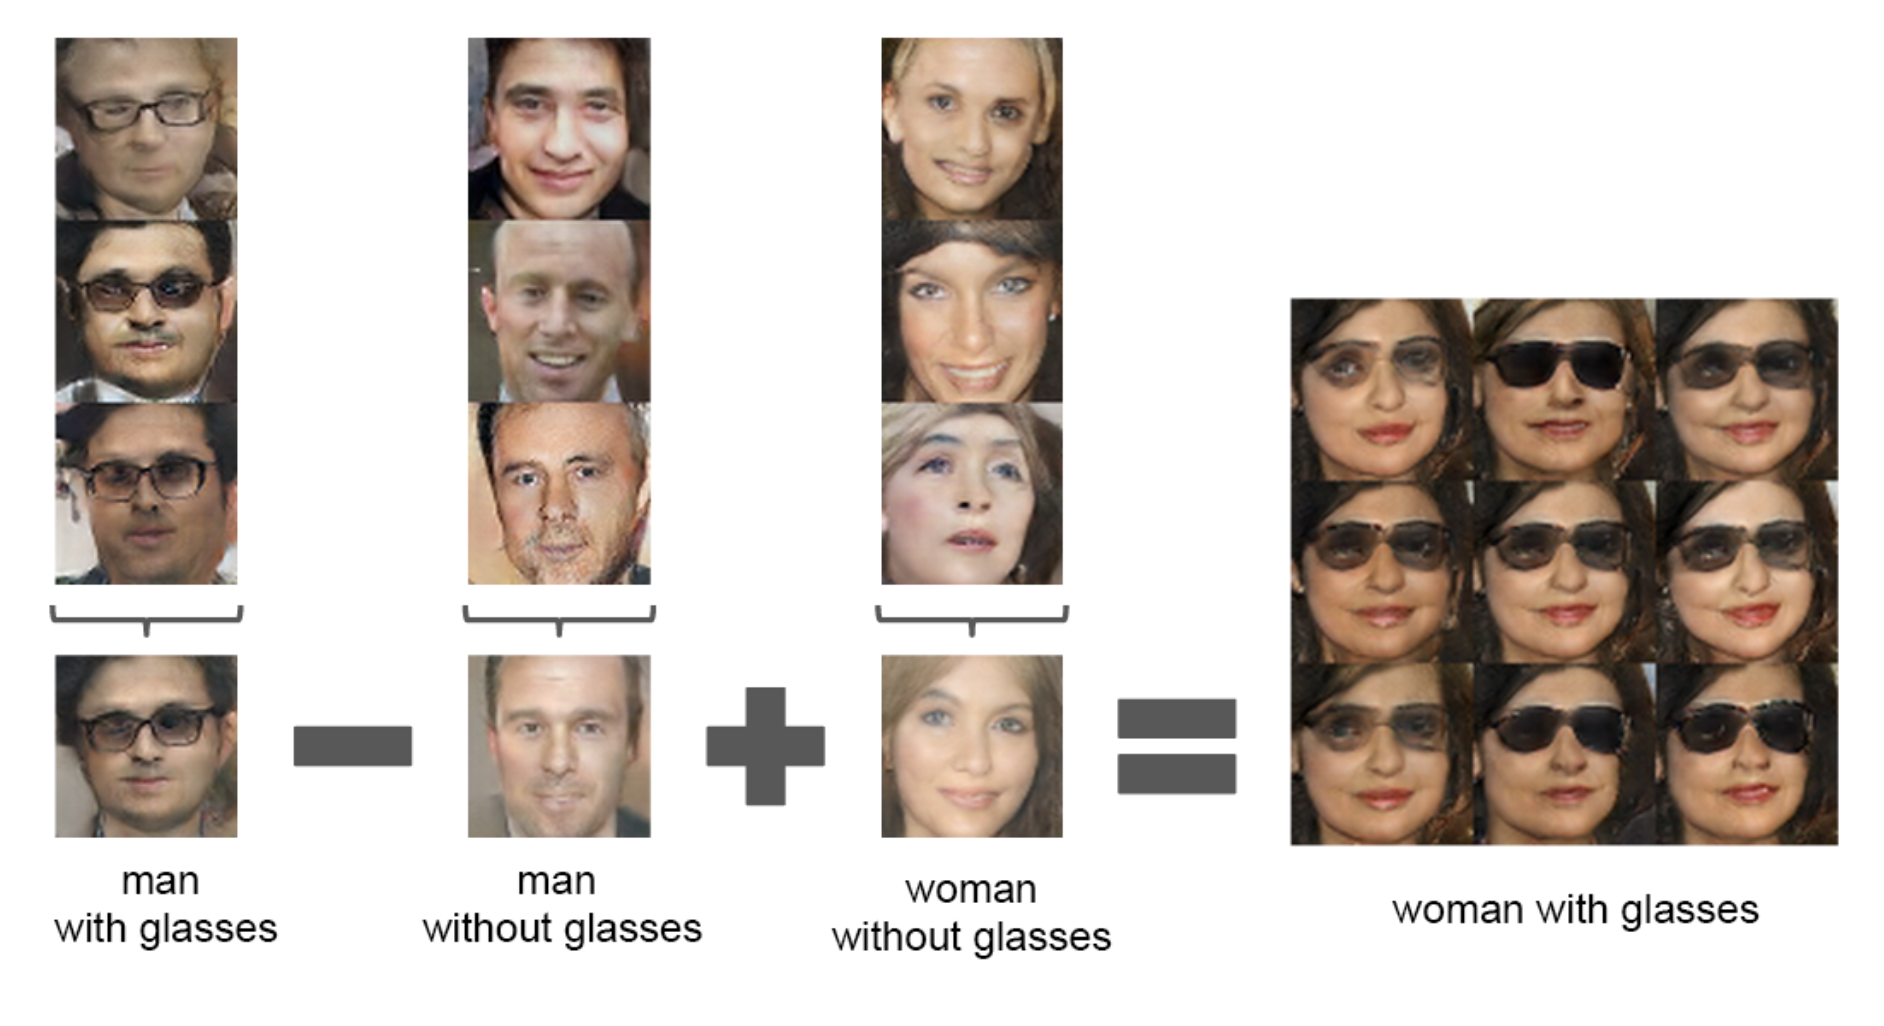
\includegraphics[scale=0.15]{woman-with-glasses}
\end{frame}

%------------------------------------------------

\section{Learning representations}

%------------------------------------------------
\begin{frame}
\frametitle{Filters that show representation learning}
\begin{tiny}
The authors did some processing on the first 6 convolutional features of the
last convolutional layer of their DCGAN's discriminator to create the image below.  
This is proof that the discriminator  is learning features.  Note on the
left-hand side taken before training that the pictures look like entire bedrooms,
but after training the pictures have key portions of a bedroom scene, like windows
and beds.  It is as though the model gets to have an idea of what things constitute
a bedroom!
\end{tiny}
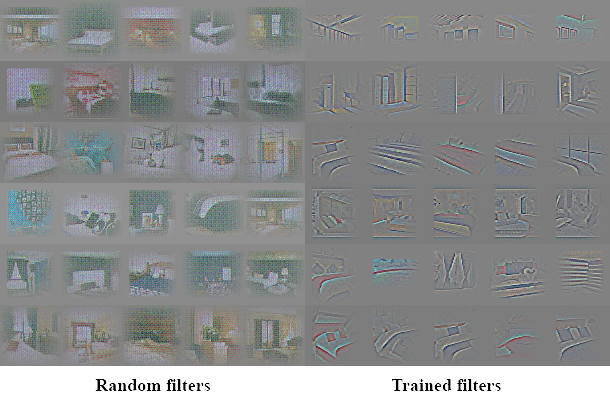
\includegraphics[scale=0.35] {feature-maps}
\end{frame}

\section{Details on fractionally-strided convolutions}
\begin{frame}
\frametitle{Details on fractionally-strided convolutions}
\begin{itemize}
\item The code for this paper, as well as many others in the references and
that one may find in the course of research, is on Github in the dcgan\_code
project \cite{dcganCode}.

\item We found that this is not compatible with the current version of Theano that
  is available to us.  
\item However the dcgan\_code Github project has a link
to the DCGAN-tensorflow \cite{dcganTf} project that we find more accessible.
\end{itemize}
\end{frame}

%------------------------------------------------


\begin{frame}
\frametitle{Fractionally-strided convolutions}
\begin{itemize}

\item The generator uses convolutional layers that we find called
deconvolutional layers in the source code that accompanies this paper
\cite{dcganCode}, and elsewhere, but that in the paper the authors write that
we should prefer the term ``\textit{fractionally-strided}.''  

\item The computations that comprise fractionally-strided convolutions are not
clear to us from the paper or the source code that accompanies it.  

\item We find the source code unclear because the authors implement
  fractionally-strided convolutions using library functions, the source code of
  which we run out of time to peruse.  The paper lacks detail on how to compute a
  fractionally-strided convolutions.
\end{itemize}
\end{frame}

%------------------------------------------------

\begin{frame}
\frametitle{Fractionally-strided convolutions}
\begin{itemize} 
  \item On the other hand, the github project \cite{dcganCode}
  that accompanies the paper \cite{repLearnDcgan} links to a Tensorflow
  implementation of the same code: \cite{dcganTf} where the author of this code
  implements fractionally-strided convolutions using Tensorflow's
  conv2d\_transpose.  
    
  \item We did some internet searching and found \cite{convArith}.
  \begin{itemize} 
    
  \item This reference plus using conv2d\_transpose in a small
      example helps us understand precisely how the fractionally-strided convolution
      operation works.  
    
      \item We feel confident to rely on conv2d\_transpose because
      the authors of the paper \cite{repLearnDcgan} we review here provide a link to
      the code in \cite{dcganTf} in their own code. 
          
      \item We feel the authors of the DCGAN's paper's endorsement of the
      Tensorflow code means conv2d\_transpose is a valid method for doing what the
      authors of \cite{repLearnDcgan} refer to as fractionally-strided convolutions,
      and that a good understanding of conv2d\_transpose is a good understanding of
      fractionally-strided convolutions.  
   \end{itemize} 
\end{itemize}
\end{frame}

%------------------------------------------------

\begin{frame}
\frametitle{Fractionally-strided convolutions}
We found some example code, and a great diagram from a StackExchange.com discussion 
\cite{stackExConv}. That explains in detail how conv2d\_transpose works.
This is the diagram we found:

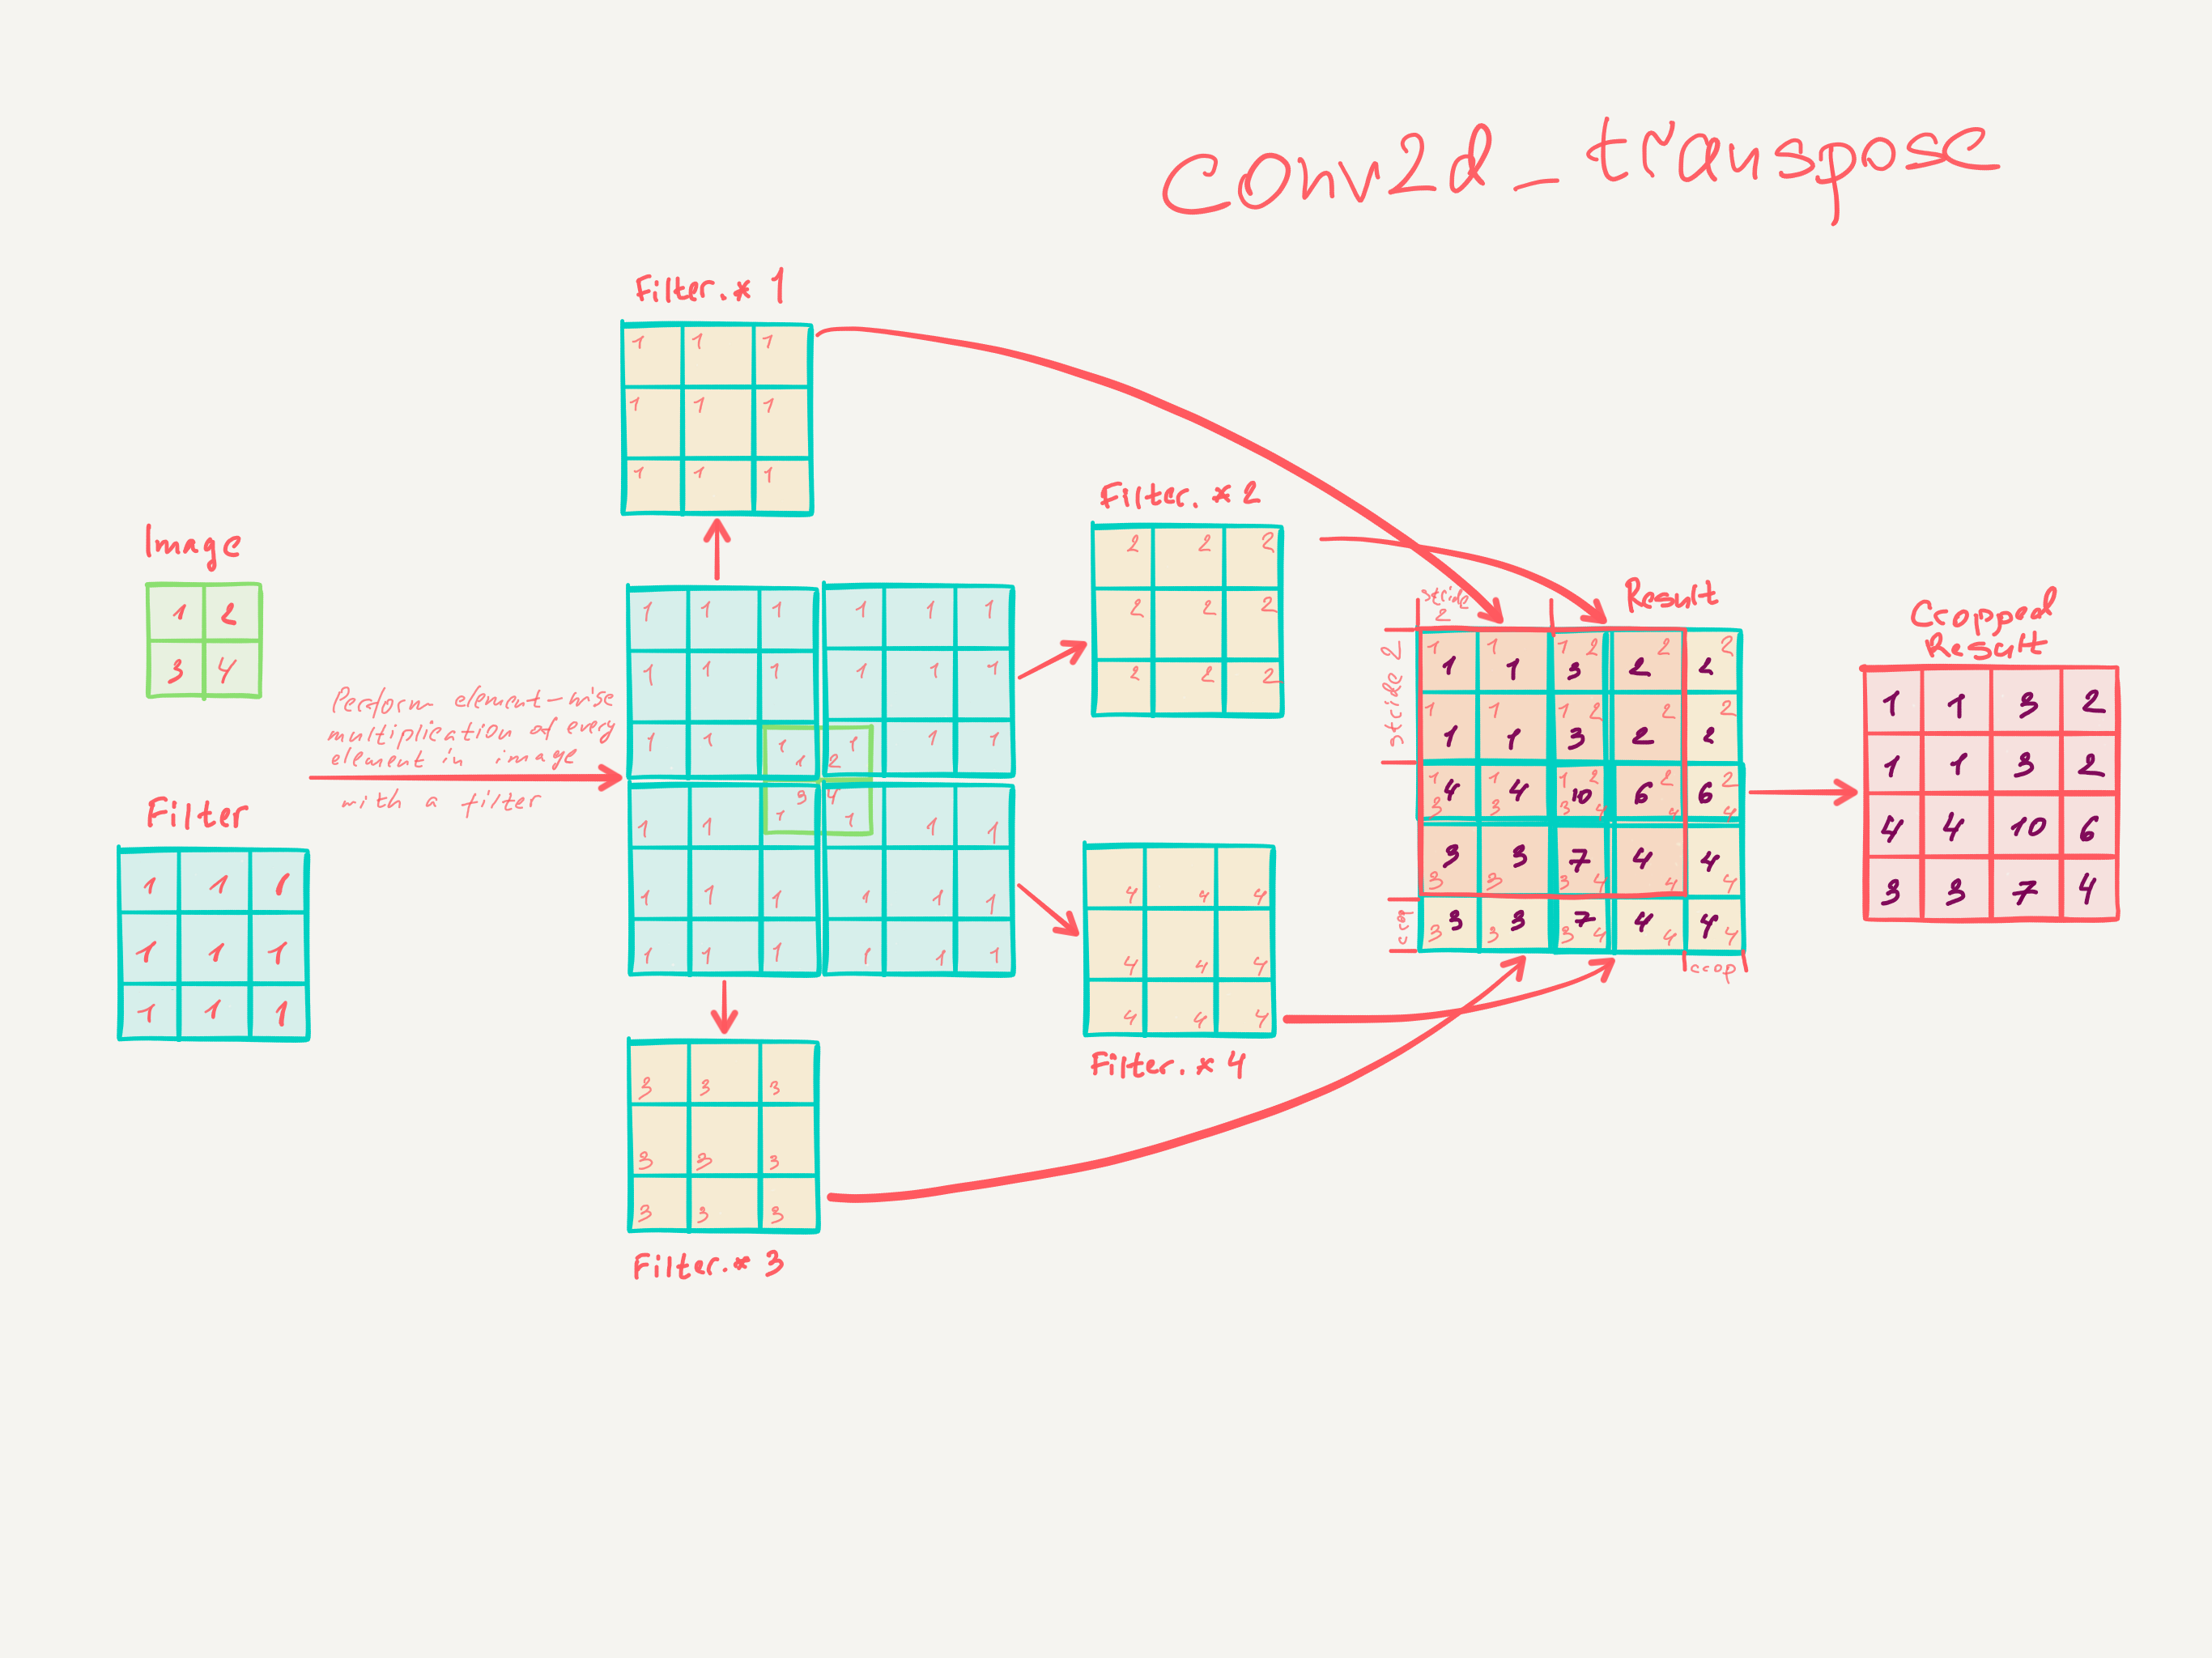
\includegraphics[scale=0.25] {conv2d_transpose-example}


In the interest of time we will not go over the code for the example, but we
will give some highlights.

\end{frame}

%-----------------------------------------------
\begin{frame}
\frametitle{Fractionally-strided convolutions}
\begin{itemize}
\item Since anyone might write anything in online discussion forums, we decided to 
confirm that Tensorflow's conv2d\_transpose operation works as the digram implies.
conv2d\_transpose has three important parameters: input tensor, 
filter, and stride. 

\item One should be careful not to confuse the term filter we
have for conv2d\_transpose and the filters that the authors of the DCGAn's paper
show on page 9. 

\item In the context of the DCGAN paper it is better to think of the filter
parameter of conv2d\_transpose  as a kernel for the conv2d\_transpose operation,
and the filter is the result of applying conv2d\_transpose to the input tensor. 
\end{itemize}
\end{frame}

%------------------------------------------------

\begin{frame}
\frametitle{Fractionally-strided convolutions}
\begin{itemize}

\item The next slide shows  a 4x4  input tensor, and the result of applying 
conv2d\_transpose to that tensor, with stride of 1,4,4,1. 

\item Conv2d\_transpose operates on 4 dimensional tensors, so we must embed the  4x4
matrix in a 4-dimensional tensor, and stride through it accordingly. Note on the 
next slide how most entries in the output tensor are copies of entries in the input
tensor, except where the 5x5 kernels must overlap in order to achieve the 
16x16 output.
\end{itemize}
\end{frame}

%------------------------------------------------

\begin{frame}
\frametitle{Fractionally-strided convolutions}
The input tensor:
\[
\begin{bmatrix}
  1 & 2 & 3 & 4 \\
  5 & 6 & 7 & 8 \\ 
  9 & 10 & 11 & 12 \\
  13 & 14 & 15 & 16
\end{bmatrix}
\]
The output we can see the entries in the input matrix copied into 5x5 intermediate
tensors and then added according to the stride of 4, and values are added when
we have overlap.  We show a screen shot to prove the code runs.

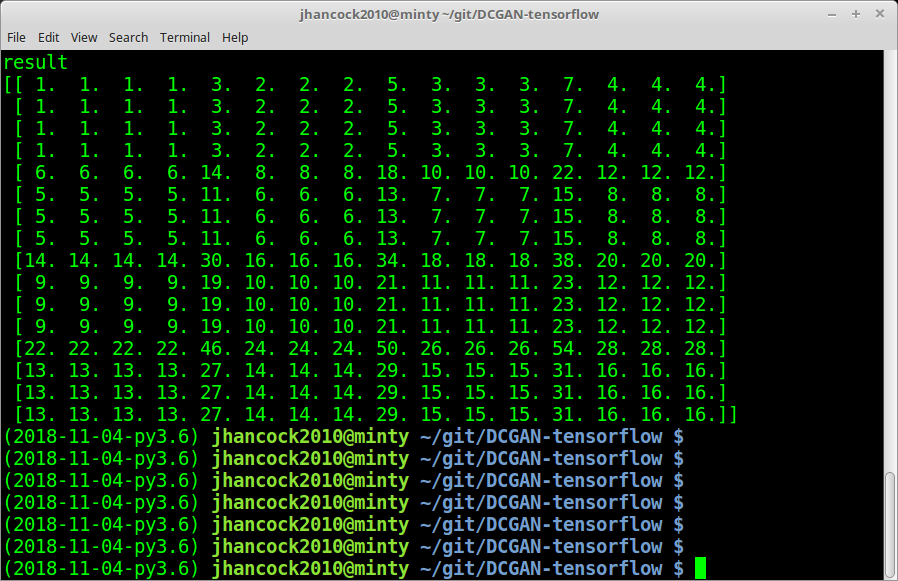
\includegraphics[scale=0.25]{conv2d-result}

\end{frame}

%------------------------------------------------

\begin{frame}
\frametitle{Fractionally-strided convolutions}

\end{frame}

%------------------------------------------------
% https://ieee-dataport.org/sites/default/files/analysis/27/IEEE%20Citation%20Guidelines.pdf

\begin{frame}[allowframebreaks]
\frametitle{References}
\footnotesize{
\begin{thebibliography}{99} % Beamer does not support BibTeX so references must be inserted manually as below

\bibitem{repLearnDcgan} S. Chintala, L. Metz, and A. Radford, 
Unsupervised representation learning with deep convolutional generative 
adversarial networks.  2016. [Online]. Available: arXiv:1511.06434v2 [cs.LG]

\bibitem{dcganCode} S. Chintala, L. Metz, and A. Radford, dcgan\_code. (2016,
May).  Available: \url{https://github.com/Newmu/dcgan\_code}. [Accessed Nov. 19,
2018].

\bibitem{lsunDataset} Large Scale Scene Understanding Challenge (2017, July).
Available: \url{http://lsun.cs.princeton.edu/2017/}. [Accessed Nov. 19, 2018].

\bibitem{dcganTf} T Kim. (2018, August).  Available: \url{https://github.com/carpedm20/DCGAN-tensorflow}. [Accessed Nov. 19, 2018].


\bibitem{gan} Y. Bengio, A. Courville,I. Goodfellow, M. Mirza, S. Ozair,  
J. Pouget-Abadie,  D. Warde-Farley, B. Xu, Generative adversarial nets. 2014. 
[Online]. Available: arXiv:1406.2661v1 [stat.ML]

\bibitem{word2Vec} T. Mikolov, I. Sutskever, K. Chen, G. Corrado, J. Dean,
``Distributed Representations of Words and Phrases and their Compositionality,''
Advances in Neural Information Processing Systems 26 (NIPS 2013), 2013. 
[Online] Available: \url{http://papers.nips.cc/paper/5021-distributed-}representations-of-words-and-phrases-and-their-compositionality.pdf

\bibitem{slidetemplate} Creodocs Limited,``Beamer Presentation,''
\emph{latextemplates.com}, 2018. [Online], Available: 
\url{http://www.latextemplates.com/templates/presentations/1/presentation\_1.zip}. [Accessed Nov. 10, 2018].

\bibitem{ieeeStyle} IEEE, Piscataway, NJ, USA. \emph{IEEE Editorial Style Manual}. 2016.
[Online]. Available: \url{http://ieeeauthorcenter.ieee.org/wp-content/uploads/IEEE\_Style_Manual.pdf}, [Accessed Nov. 11, 2018].

\bibitem{unsupVideo} Y. LeCun, ``Unsupervised Representation Learning,''
2017. Accessed on: Nov 11, 2018. [online]. Available: \url{https://www.youtube.com/watch?v=ceD736_Fknc}  

\bibitem{deepLearnR} F. Chollet, and J.J. Allaire.  
\textit{Deep Learning with R}. Manning Publications 2018. [E-Book] Available: Safari
E-Book.

\bibitem{deepLearnBookGenCh} Y. Bengio, A. Courville, I. Goodfellow. (2016). ``Chapter 20 Deep Generative Models,'' 2016. [Online] Available: \url{https://www.deeplearningbook.org/contents/generative_models.html}. [Accessed: Nov. 20, 2018].

\bibitem{ganList} A. Hindupur, ``A list of all named GANs!'' github.com, Sep. 30,
2018. [Online]. Available: \url{https://github.com/hindupuravinash/the-gan-zoo}. 
[Accessed Nov. 21, 2018]. 

\bibitem{lenet5} L. Bottou, P. Haffner, Y. Bengio, Y. LeCun, ``Gradient-Based Learning
Applied to Document Recognition,'' Proc of the IEEE, Nov., 1998. [Online]. Available:
\url{http://yann.lecun.com/exdb/publis/pdf/lecun-01a.pdf}. [Accessed Nov. 21, 2018].

\bibitem{convArith} V. Dumoulin and F. Visin, ``A guide to convolution arithmetic for 
deep learning,'' Jan 2018. [Online]. Available: Github, https://github.com/vdumoulin/conv\_arithmetic.  [Accessed November 21, 2018].

\bibitem{stackExConv} Stack Exchange user Andriys, ``What are deconvolutional layers,''
datascience.stackexchange.com, answer written July 14 2017, edited Nov. 19, 2017. 
[Online]. Available: 
\url{https://datascience.stackexchange.com/questions/6107/what-are-deconvolutional-layers}. 
[Accessed Nov.  22, 2018].

\bibitem{cnnlecture} Xingquan Zhu. 2018. Convolutional Neural Networks (CNN) retrieved
 October 22, 2018 from \url{https://canvas.fau.edu/files/14310707/download?download\_fr
d=1}

\end{thebibliography}
}
\end{frame}

%------------------------------------------------

\begin{frame}
\Huge{\centerline{The End}}
\end{frame}

%----------------------------------------------------------------------------------------

\end{document} 
